\documentclass[main.tex]{subfiles}
\begin{document}

\section{Definitie Riemannintegraal}
\label{sec:defin-riem}

\begin{de}
  Een \term{verdeling} van een interval $\interval{a}{b}$ is een verzameling $P = \{x_{0},x_{1},\dotsc,x_{n}\}$ met $a = x_{0} < x_{1} < \dotsb < x_{n-1} < x_{n} = b$.
\end{de}

\begin{de}
  We noemen een verdeling $P'$ \term{fijner} dan een verzameling $P$ als $P$ een deel is van $P'$.
\end{de}

\begin{st}
  Zij $P_{1}$ en $P_{2}$ twee verdelingen van een interval $\interval{a}{b}$, dan bestaat er steeds een verdeling $P$ van $\interval{a}{b}$ zodat $P$ fijner is dan $P_{1}$ en fijner dan $P_{2}$.

  \begin{proof}
    Kies $P = P_{1} \cup P_{2}$.
    \question{dat was te makkelijk?}
  \end{proof}
\end{st}

\begin{de}
  Zij $f:\ \interval{a}{b} \rightarrow \mathbb{R}$ een begrensde functie gedefinieerdop een gesloten begrensd interval en zij $P = \{x_{0},\dotsc,x_{n}\}$ een verdeling van het interval $\interval{a}{b}$.
  We definieren de \term{ondersom} $\underline{S}(f,P)$ als volgt:
  \[ \underline{S}(f,P) = \sum_{k=1}^{n} (x_{k}-x_{k-1}) \inf\{ f(x) \mid x\in \interval{x_{k-1}}{x_{k}}\} \]
  We definieren de \term{bovensom} $\overline{S}(f,P)$ als volgt:  
  \[ \overline{S}(f,P) = \sum_{k=1}^{n} (x_{k}-x_{k-1}) \sup\{ f(x) \mid x\in \interval{x_{k-1}}{x_{k}}\} \]
\end{de}

\begin{opm}
  Merk op dat de onder- en bovensom goed gedefinieerd zijn omdat $f$ begrensd is.
\end{opm}

\begin{bpr}
  Zij $f:\ \interval{a}{b} \rightarrow \mathbb{R}$ een begrensde functie en $P$ een verdeling van $\interval{a}{b}$, dan is de ondersom kleiner dan de bovensom.

  \begin{proof}
    Dit is een rechtstreeks gevolg van het feit dat het supremum van een verzameling groter is dan, of gelijk aan, het infimum van die verzameling.\stref{st:infimum-kleiner-dan-supremum}
  \end{proof}
\end{bpr}

\begin{bpr}
  Zij $f:\ \interval{a}{b} \rightarrow \mathbb{R}$ een begrensde functie en $P$ en $P'$ verdelingen van $\interval{a}{b}$ zodat $P'$ fijner is dan $P$, dan geldt het volgende:
  \[ \underline{S}(f,P) \le \underline{S}(f,P') \text{ en } \overline{S}(f,P') \le \overline{S}(f,P) \]

  \begin{proof}
    Het volstaat om de situatie te bekijken waarin $P'$ precies \'e\'en punt $y$ meer bevat dan $P$.
    Het punt $x$ zit tussen precies twee punten, zeg $c$ en $d$ (stel $c<d$), van $P$.
    Omdat de rest gelijk blijft, bekijken we het deel dat rond die punten draait:
    \[ \inf\{ f(x) \mid x\in \interval{c}{d}\} (c-d) \le \inf\{ f(x) \mid x\in \interval{c}{y}\} (c-y) + \inf\{ f(x) \mid x\in \interval{y}{d}\} (y-d)\]
  \end{proof}
    \[ \sup\{ f(x) \mid x\in \interval{c}{d}\} (c-d) \ge \inf\{ f(x) \mid x\in \interval{c}{y}\} (c-y) + \sup\{ f(x) \mid x\in \interval{y}{d}\} (y-d)\]
\end{bpr}

\begin{de}
  Zij $f:\ \interval{a}{b} \rightarrow \mathbb{R}$ een begrensde functie.
  De \term{onder-Riemannintegraal} $\underline{S}$ van $f$ over $\interval{a}{b}$ definieren we als volgt:
  \[ \underline{S} = \sup\left\{\underline{S}(f,P) \mid P \text{ is een verdeling van } \interval{a}{b} \right\} \]
\end{de}

\begin{de}
  Zij $f:\ \interval{a}{b} \rightarrow \mathbb{R}$ een begrensde functie.
  De \term{boven-Riemannintegraal} $\overline{S}$ van $f$ over $\interval{a}{b}$ definieren we als volgt:
  \[ \overline{S} = \inf\left\{\overline{S}(f,P) \mid P \text{ is een verdeling van } \interval{a}{b} \right\} \]
\end{de}

\begin{de}
  We noemen een begrensde functie $f:\ \interval{a}{b} \rightarrow \mathbb{R}$ \term{Riemannintegreerbaar} als $\underline{S}(f) = \overline{S}(f)$ geldt.
  In dit geval noemen we deze waarde de \term{Riemannintegraal} van $f$ over $\interval{a}{b}$.
  We noteren dit dan als volgt:
  \[ \int_{a}^{b}f \quad\text{ of }\quad \int_{a}^{b}f(x)\ dx \]
\end{de}

\begin{tvb}
  Niet elke functie is Riemannintegreerbaar.

  \begin{proof}
    Kies de functie $f$ als volgt:

    \noindent
    \begin{minipage}{.45\textwidth}
      \begin{figure}[H]
        \centering
        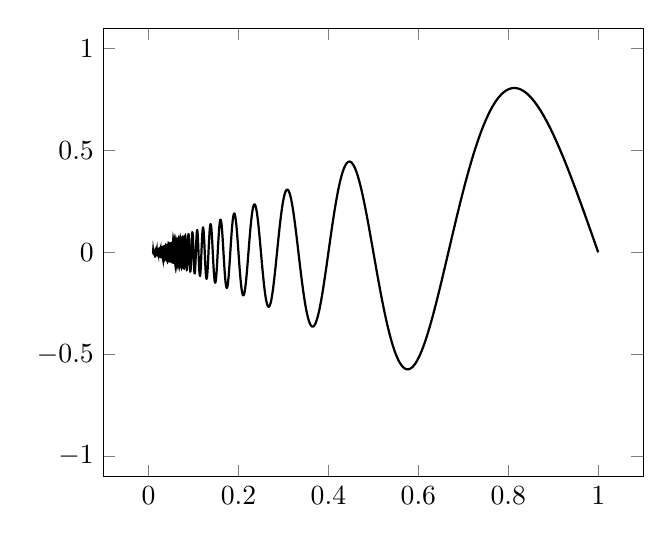
\begin{tikzpicture}
          \begin{axis}[ymin=-1.1, ymax=1.1, xmin=-0.1, xmax=1.1, no markers]
            \addplot[samples=5000,thick,domain=0.01:1]{x*sin((1/x)*360)};
          \end{axis}
        \end{tikzpicture}
      \end{figure}
    \end{minipage}
    \begin{minipage}{.45\textwidth}
      \[ x \mapsto \frac{1}{x}\sin\left(\frac{1}{x}\right) \]
    \end{minipage}

    \noindent(Merk op dat deze functie zelfs fout getekend wordt omdat de numerieke benadering die de computer (die dit tekent) probeert te maken niet nauwkeurig genoeg is. Naar $0$ toe begint te grafiek oneindig snel te oscileren.)
    \TODO{bewijs dat deze functie inderdaad niet integreerbaar is}
  \end{proof}
\end{tvb}

\begin{st}
  \stiekem{Juni 2014}
  Zij $f:\ \mathbb{R} \rightarrow \mathbb{R}$ een continue functie, dan is $f$ de constante nulfunctie als en slechts als $f$ de volgende eigenschap heeft:
  \[ \forall \interval{a}{b} \subseteq \mathbb{R}:\ \int_{a}^{b}f(x)\ dx\]

  \begin{proof}
    \noindent
    \begin{itemize}
    \item $\Rightarrow$\\
      Kies willekeurig $\interval{a}{b}\subseteq \mathbb{R}$.
      Voor elke verdeling van $\interval{a}{b}$ is zowel de bovensom als de ondersom nul en dus ook de integraal.
    \item $\Leftarrow$\\
      Bewijs uit het ongerijmde: Stel dat $f$ niet de nulfunctie zou zijn.
      Er bestaat dan een $c\in\mathbb{R}$ zodat $f(c)$ niet nul is.
      Veronderstel dat $f(c)$ positief is (het andere geval is immers geheel analoog).
      Omdat $f$ continu is, bestaat er een omgeving van straal $\delta\in\mathbb{R}_{0}^{+}$ rond $c$ waarin $f$ strikt groter is dan $\frac{f(c)}{2}$:
      \[ \forall x \in B(c,\delta):\ f(x) > \frac{f(c)}{2} \]
      Beschouw nu het interval $\interval{x-\frac{\delta}{2}}{x+\frac{\delta}{2}}$.
      De integraal van $f$ over dit interval is strikt groter dan $\frac{\delta f(c)}{2}$ en dus niet precies nul.
      Contradictie.
    \end{itemize}
  \end{proof}
\end{st}

\begin{tvb}
  \stiekem{Juni 2014}
  Bovenstaande stelling geldt niet als $f$ niet continu hoeft te zijn.

  \begin{proof}
    Beschouw de functie $g$ als volgt:
    \[
    g:\ \mathbb{R} \rightarrow \mathbb{R}:\ x \mapsto
    \begin{cases}
      1 &\text{ als } x = 0\\
      0 &\text{ als } x \neq 0
    \end{cases}
    \]
    $g$ is Riemann-integreerbaar met overal integraal $0$ maar is niet de nulfunctie.
  \end{proof}
\end{tvb}

\end{document}

%%% Local Variables:
%%% mode: latex
%%% TeX-master: t
%%% End:
